\chapter{Our Trip to Israel, 1984}\label{Israel}


\section{June 4th}

Tony and I left Johannesburg at 9~pm on the long flight to Tel
Aviv. We flew South African Airways which involved flying the long way
round stopping at Lisbon and Rome \textit{en route}. I am delighted
that I have not only overcome my fear of flying but that I actually
enjoy it! I wonder why?

\section{June 5th}

We arrived in Tel Aviv at 2.30~pm and were met at the airport by Amir
Gidron and his small daughter.  He took us to the Sheraton Hotel, a
lovely hotel where we had a delightful room in the Gold Carpet
section, (1704) relaxed after the 20 hour flight and had a light
supper. testgsa

\section{June 6th}

We had quite a long walk in the morning and saw a little of our end of
Tel Aviv. It is a scruffy place with no attention being paid to
tidiness or the cultivation of small parks etc: and, if it were not
for the glorious 2i mile - long beach, it would have little to
offer. The Mediterranean Sea runs the entire coast of Israel. Had
lunch and watched a video in the afternoon. sdfasd

We took a taxi to Old Jaffa in the early evening. This is a
fascinating place, reminiscent of the narrow streets and the ``nooks
and crannies'' of places we have been to in Turkey. Full of atmosphere
with dark little streets and alleys where Art Galleries and
restaurants would have been doing a roaring trade if it had not been a
public holiday. Before Independence Old Jaffa was occupied by Arabs so
it was, naturally, allowed to become very run-down but the dilapidated
buildings are slowly being restored.

I would not have fancied any of the food being served in the
restaurants which were open because the meat etc, was displayed on
tables on the streets; perhaps I am more fastidious than I used to be
as we saw a lot of this sort of thing in Turkey. A really balmy night
with a light breeze -- how lovely to feel warm after the cold of
Johannesburg! -- The view back to Tel Aviv was enchanting. The taxi we
had booked was waiting for us and we went back to the hotel and had
dinner in the ``Twelve Tribes'' restaurant -- very restful and almost
sepulchral. We had a lovely meal; all the restaurant people were very
pleasant and remembered Tony who seems to be as much at home here as
he does everywhere else.

\section{June 7th}

Before getting up, we could hear the ``pit-pat'' of the bat and ball
game the Tel Avivians play on the beach. It is very popular and sounds
like thousands of horses hooves.

We took a taxi to Beth Hatefutsoth the Museum of the Jewish
Diaspora. This was an enlightening experience. We were there for
2~hours but understood why it is recommended that one should spend
6~hours there.

This is the story of the endless struggle for survival of the
Jews. Diaspora means scattering and the Jews have been scattered to
the corners of the earth. The story is told of the struggle to be
allowed to practice their own religious beliefs through the centuries
but, above all, to be allowed to return to the promised land. What a
story! A lesser nation would not have survived but, because of the
steadfast resolve and resilience of these people and the belief in
their own destiny, they have risen up again and again since the
beginning of time. Religion and belief are the basis of their lives
and history.

The torment, suffering and harassments are depicted by means of
visual and aural aids, the great achievements of the sons and
daughters of this fine nation. We saw many pictures and photographs of
those who have left an indelible mark upon the world -- Musicians,
Authors, Doctors, philosophers to name only a few professions and one
is made to realise once more, what remarkable people the Jews are;
surely they must be the chosen people by virtue of their supreme
talents in so many walks of life but then if so, why have they been
made to suffer so through the centuries? I expected to see more of the
terrible holocaust but that was to come later. It was a very moving
experience to visit this museum: everything is clearly and beautifully
presented in a magnificent building which is in the University
Grounds.

After lunch we rested and then took a walk along the promenade when it
was cooler. The weather was superb and the beach crowded.

In the evening Amir Gidron and his wife collected us and took us to Old
Jaffa where we had a delightful fish supper in their favourite
restaurant. We enjoyed their company and I was, once more, fascinated
by the atmosphere of Old Jaffa. Back in Tel Aviv we had another little
walk along the promenade before going to bed - another warm night, glad
of the hotels air-conditioning.

\section{June 8th}

Another lovely warm day and, once more, the beach is crowded from
early morning.

Today is auspicious!

We go ``unto Jerusalem''!

I feel I have been building up to this moment.  I have looked forward
to this and to seeing some of the countryside outside Tel Aviv.

We left Tel Aviv by taxi at 2.30~pm.

The ride was enjoyable and there was very attractive countryside on
each side of the highway. We passed the Monastery of Latrun to our
right where the Monks keep a vow of silence. Imagine never saying
anything!

I must admit to a tremendous sense of disappointment upon not seeing
the panoramic view of Jerusalem I expected as we approached;
apparently this is the wrong approach road for this. Coming into
Jerusalem we saw several burned out wrecks of army vehicles which have
been deliberately left by the roadside as reminders of the War of
Independence in 1948.

Jerusalem is a city of hills and these hills and the surrounding
countryside are just as I have always imagined. Our hotel is Laromme
-- a new, very comfortable one with welcome air-conditioning.

After unpacking, we took a little walk past the King David Hotel and
from there, we saw the view I have been waiting for -- the Old City. A
friend of mine thought Jerusalem to be the ugliest city she had ever
seen. To my mind, it is one of the most beautiful and memorable and I
do not believe I think in this way just because of the association of
ideas. I feel I have been here before!

We saw a small area dedicated to the memory of Sir Moses Montefiore --
we even saw the carriage he had used -- he was a great benefactor to
the Jewish nation.

Back at the hotel the arrangements were very much geared to the
Sabbath (Shabbat) dinner which takes place on Friday evenings. After
this the Orthodox Jews spend all day Saturday in peace and quiet and
reading the five books of Moses but the Friday evening meal is very
special to them and usually only includes members of the
family. Several people were celebrating Shabbat in the hotel dining
room including 2 large families. It did not seem to matter too much
that younger members of the families were not paying much attention to
the proceedings! One is supposed to use only one of the lifts on
Shabbat and this would have been acceptable if things had been a little
better organised but that lift did not seem to work half the time.

\section{Shabbat}

We had a typical Israeli breakfast -- more like lunch really but you
can manage to find the cornflakes and milk, glorious fruit
(strawberries!) bread rolls etc: amidst the tremendous array of fish,
eggs, cheese, pate, salads (spring onions for breakfast!!) yoghurt
etc. People complain about the Israeli breakfasts but I thought they
were fun.

Teddy Vardi picked us up at 8.30~am. He is to be our guide for the
next 2 or 3 days. Such an interesting personality, speaks several
languages and English with an American accent.

Since this would have been a quiet day in Jerusalem with many places
closed, we went to Masada and the Dead Sea on the first day.

Out of Jerusalem, we passed through Bethany where lived Mary, Martha
and Lazarus. We saw the Hills of Moab where Ruth came from (``Thy
people shall be my people...whither thou goest'') Approached then the
hills and desert of Judea and passed on our right the Inn of the Good
Samaritan - although Teddy said that a Samaritan would never have been
on the road in a million years. However, he said it was
``traditional'' as so many things seemed to be ``traditional'''. We
saw Jericho in the distance on the left. This is very cruel terrain
and must indeed look very much the same as it did in those far off
days but it does possess a majestic beauty.

Teddy pointed out a kibbutz as we approached the Dead Sea area. We had
dropped down 1300 feet below sea level and the soil is full of
minerals and salt which, of course, would make the growing of
vegetables etc. extremely difficult. Nevertheless, the young people on
this kibbutz have washed the soil 4 times to rid it of harmful
deposits and have successfully grown fields of grapes, olives, corn
etc.: splashes of welcome green in the middle of the arid desert. What
an achievement and what back-breaking-work must have gone into it but
these people have such an ideal. Who else would make a desert grow!
The Dead Sea, on our left looked tranquil and beautiful but of course,
there is nothing living in it. It is possible for anyone to float on
the water and never drown -- want a bet?

We drove alongside it for many miles and beyond saw the hills of
Jordan. The Dead Sea is 11 miles wide at its widest point. On our
right we saw Qumran and looked across at the caves where the Dead Sea
Scrolls were found. They had been preserved in jars and hidden there
by the Essenes (John the Baptist was an Essene) when they hid from the
Romans. David fled from Saul to a place nearby called Einged and hid
in the hills there.

We arrived in Masada -- this fortress built by Herod is awesome and
huge. We went to the top by cable car. Such intense heat but very,
very dry. It was fabulously interesting to see the ruins of this once
mighty fortress and palace -- built because Herod was afraid of
everyone and wanted somewhere safe to barricade himself in, in fact he
lived there for only 2 days. The genius and energy of the builders can
only be wondered at -- there were hanging gardens, a swimming pool, an
elaborate bath-house, vast stores, a synagogue and ritual baths,
everything being protected by sentry towers set at intervals along an
encircling wall. Approach was difficult. The only way seems to have
been by the ``Snake Path'' which winds up the eastern side of the
mountain. One can see the remains of Roman camps from the top of the
mountain. After the fall of Jerusalem in 70~CE, a group of 960 Jewish
Zealots (men, women and children) barricaded themselves in on Masada
and held it for 2-3~years (although Teddy told us it was only for 1
year). When conquest seemed imminent and the Romans were ready to
burst in -- having built a ramp -- Eleazar ben Yair spoke to the
Zealots and told each man to kill his wife and children then to choose
10 men to kill all the rest and, in that way, the Romans did not find
anyone alive. Teddy said that in fact there were 2 women and three
children who survived and in retrospect, someone must have told the
story. Ample food stores were left to prove to the Romans that it was
not because of lack of food and provisions that nobody was found
alive.

The atmosphere of this place was terrific, full of history and
interest, I longed for a curtain to be drawn back so that I could see
it exactly as it was, even if only for a few seconds. We explored for
$2 \frac{1}{2}$ hours with Teddy pointing out the places of
interest. I ruined a pair of shoes and had to buy some more in
Jerusalem but it was worth it.

Refer to more literature about Masada.

We took the road back to Jerusalem, this time with the Dead Sea on our
right and stopped for lunch at the Ein Gedi kibbutz which is on the
shores of the Sea. Afterwards we took a little walk down to the water
and put our hands into it. The water feels very oily and we were
advised to wash the water off. We were at the lowest point of the
earth.

Again we could see Jericho in the distance on our right as we started
to climb back up to Jerusalem.

Incidentally, Joshua is alleged to have knocked down the walls of
Jericho but no trace of any walls has ever been found.

Re-entering Jerusalem we saw Mount Scopus, the site of the University
and the Hadassah Medical Centre and the Mount of Olives. Contained in
the synagogue of the Hadassah Medical Centre are the Jerusalem windows
of Marc Chagall and we were later to see another superb example of his
work in the Knesset.

We saw so many interesting places on the way to Jerusalem --
everything looks and feels exactly the way I had imagined it would.

Teddy took us to see the Garden Tomb -- one of two supposed places
where the body of Jesus was laid after the Crucifixion. This one is in
a quiet and lovely garden and fits exactly the picture I have of the
place where Jesus was laid. From the garden one can look across to
``Gordon's Calvary'' where the crucifixion could have taken place
(rather than at the other traditional site in the Church of the Holy
Sepulchre) for it was General Gordon who fostered the idea that it was
here in this beautiful garden that He was laid.

I would like it to be here.

The feeling of its authenticity is so strong amongst the British that
British people come out from the U.K. to look after the shop and act
as guides in the garden.

Next we went to the Catholic Church of all Nations and saw the stone
of the agony where Jesus wept in agony before he was crucified. Next
door is the Church of the Assumption but it was closed and we could
not go in. Close by is the Garden of Gethsemane, so called because of
the words Get Shemen which mean Oil Press. An olive tree nevers dies
and there are trees here from the time of Jesus; He used to meet His
friends here and the olives must have been pressed in this garden for
the oil to be extracted. We could see across to ``St. Peter in
Gallicantu'' a church to the memory of Peter's denial of
Christ. ``Galli'' means ``cock'' and ``Cantu'' means ``sing''. We went
next to the place which used to be the centre of the City of David and
the famous spring which is there. Jerusalem is built on hills and we
could see this very well from this place. We paused to look down into
the Kidron valley which runs between the Mount of Olives and Mount
Ophel. In the valley are the ancient tombs of St James, Zachariah and
Absalom.

From the Kidron valley we looked across to the Golden Gate of the Old
City of Jerusalem through which the new Messiah must pass when he
comes. A huge graveyard covers a large area of the Kidron valley.

\section{June 10th}

Teddy picked us up at 8.30~am and we proceeded straight to the Old
City.

We had a long day ahead of us.  We walked through the Jewish and
Armenian quarters which were clean and lovely and built of the white
stone of Jerusalem.

It was with amazement that we saw the original columns of the (Roman)
Cadorna Maxima -- part of a street of Roman times -- and looked down
from the pavement to see several layers of civilization through
grilles. We seemed to arrive very quickly at the Western Wall
(sometimes referred to as the Wailing Wall), a scene of great activity
and prayer. The wall is the only remaining part of the original temple
and when Jerusalem was divided and the wall no longer belonged to the
Israelis, there was much distress amongst them.

The wall is a mighty symbol of their faith and destiny and much
significance is attached to being able to pray there.

There are small notes and messages by the thousand tucked into cracks
in the stones left there by people who believe fervently that their
prayers will be answered if they are offered up at the ``Wailing
Wall''.

I was not allowed to approach the wall with the men but went to
another place for women and I touched it. Some people were kissing it
-- all very dramatic to an English observer!

During the day Teddy pointed out to us the eight gates of the city:
Jaffa, Dung, Damascus, Lion, New, Golden, Zion and St. Stephen's.

On Mount Moriah (which used to be called Temple Mount) we visited the
exquisite El Aqsa Mosque. This is the site of the original temple of
Jerusalem which was destroyed twice. We had to remove our shoes to
enter the Mosque and the men had to cover their heads. The Mosque has
a beautiful ceiling and interior, quite lovely.

We walked across to the Dome of the Rock (sometimes wrongly called the
Mosque of Omar). The rock is the original one upon which Abraham bound
Isaac for sacrifice and the lovely building is built around it. The
rock is in the centre of the building and the building is said to be
in the centre of the earth.

From here we walked to the fortress of Antonia named after Anthony,
Herod's great friend. This is the first station of the cross and it is
where Jesus was tried by Pontius Pilate, ``Ecce Homo?'' - ``Is this
the man?''.

We walked up the Via Dolorosa - now an Arab market of great colour and
interest but moving to me all the same and full of atmosphere for this
is the way Jesus took carrying the cross upon which he was to be
crucified. The stations of the cross are indicated and two of them are
in the form of small chapels, one where He was scourged and the other
where he was committed. It was not difficult for me to imagine Him
picking up the cross and beginning His walk to Calvary (Golgotha). He
fell twice and at Station No.6, His face was wiped by a woman called
Veronica. Her names means ``True image'' and it came about because, as
she wiped His face, the image of it became imprinted on the cloth for
ever. At this 6th Station of the Cross, Teddy suddenly diverted our
attention to an interesting shop belonging to Khaidar Baidoun and
introduced us to the owner, a handsome and intelligent Arab, who was
extremely interested in South Africa. His shop is full of
archeological treasures, all of which are quite authentic. Customers
come from all over the world including Wilbur Smith from Cape Town. I
saw several relics I would like to possess but we did not know at that
stage, how the dollars would last; however, on the day before our
departure from the country, we again went back to this shop in the Old
City and Tony bought me an oil lamp and filler from the time of Jesus
(and therefore almost 2000 years old) and a Canaanite wine carafe 3000
years old - all in perfect condition and all amongst my proudest
possessions.

At the end of the Via Dolorosa is the Church of the Holy Sepulchre,
now a Catholic Church although it seemed to be generally used by many
denominations; there was a Greek Orthodox service being conducted
whilst we were there. It is extremely ornate and not characteristic of
the simplicity with which we associate Jesus and I did not like the
commercialism of the whole thing. We did not go to see the
(traditional) tomb, but it is possible to put one's hand into a hole
which is supposed to have been made by the Cross. I feel more strongly
than ever, that General Gordon was correct in his idea of where
Calvary was and that the Garden Tomb is more in keeping with our ideas
of quietness and dignity. I suppose we shall never really know.

Afterwards we visited the Church of the Dormition, where Mary who was
never known to sin, is lying in a state between Heaven and Earth -- a
beautiful tomb in a quiet and peaceful church. The contrast was even
more striking to us having been so recently to the garish Church of
the Holy Sepulchre.

We then went to Mount Zion and saw first the tomb of David, one of the
great kings of Israel -- perhaps the greatest -- which is beneath the
room where the Last Supper was held. I was not so much awed by this
room as I thought I would be, although there was a certain
atmosphere. Once more I wished I could see it all as it was then.

We left Jerusalem then with sadness on my part but I was not to know
that we would be returning to this fascinating Old City three more
times.

Teddy drove us to Bethlehem. Quite a large town. One's mind conjures
up a certain picture and, in my mind, I could only see a stable, but
of course, over the site of the stable a church has been built, the
Church of the Nativity, which again is quite ornate but beautiful in
its significance. Underneath the church is the site of the actual
birth and it was possible to picture the Holy Family with the
Shepherds and the three wise men, Caspar, Melchior and Balthazar,
worshipping the baby Jesus.

Teddy then took us to the Tomb of Rachel, wife of Jacob, who died
giving birth to Benjamin.

The entrance was guarded by 2 Israeli soldiers and, as we came out, I
was disconcerted to look upwards to a rooftop on the opposite side of
the street to see another soldier with his machine gun pointing
directly at me! Nobody was able to explain why this tomb is so heavily
guarded and we saw no other place, apart from the Knesset, with such
close military protection. The military preparedness of Israel is a
well-known situation but tension and incidents were not obvious to us
on this tour.

On the way back to Jerusalem we passed by the ``Fields of the
Shepherds'' on the right. This is where the shepherds saw the angels
who told them the news of Jesus' birth. Close by here, Ruth gleaned
corn in the fields of Boaz whom she later married.

It was lovely to go back into Jerusalem again and, once more, I had
the feeling of intimacy with the place. There are several new housing
developments on the hills of Jerusalem although ft is difficult to
imagine how anyone can afford a house in Israel with the cost of
living so high and ever climbing. Incidentally, one of the many hills
is called ``The Hill of Evil Counsel'' it could be a mere coincidence
that, upon this hill the United Nations have their headquarters!

Soon we passed by the Valley of the Cross from where the tree which
was to provide the wood for the cross was felled. There are a church
and a monastery there now.

Our next visit on this crowded day, was to the Israeli Museum and the
Shrine of the Book wherein some of the original Dead Sea Scrolls are
kept in the most perfect conditions and temperatures. It was
incredible to see these parchments as well as kitchen utensils and
woven baskets in such a wonderful state of preservation.

When the Essenes escaped from Jerusalem in the time of the Romans,
they took the Scrolls -- the original laws of Moses and the Old
Testament books of Moses from the Bible -- and in order to keep them
preserved they stored them in Jars. The shape of the lid of the Jar is
the shape of the roof of the Shrine of the Book, but until that is
explained to the visitor, the building does look to be a peculiar
shape. The Essenes went to live in the Judean desert at Qumran and
there they learned to exist away from the Roman tyranny.

Back in Jerusalem, Teddy took us to the Yad Vashem at Mount
Herzl. This is a necessary monument to the 6,000,000 Jews who perished
in the Holocaust. Astonishing works of art in stone welcome the
visitor at the entrance to the building and one must stop and admire
the depiction of the diaspora, Holocaust, the rising up again and the
return of the Jews to their very own land.

The pictures, photographs and movie and the entire atmosphere of the
Yad Vashem are heartbreaking in the extreme and one is brought to
tears by this terrible example of Man's inhumanity to Man not least
because it seems that the world stood by with full knowledge of it and
did nothing to help.

The story of the Jews of Warsaw who were kept in the Warsaw Ghetto
under appalling conditions of cold, starvation, torture and death, is
a terrible one and the pictures of the children are, as usual, the
most moving.

Thank goodness that most of the Gestapo and S.S. torturers have been
brought to trial and death because of their dreadful crimes.

We were horrified to see a guitar and a pair of shoes which a prisoner
had been forced to make from his copy of the sacred Torah. One can
only begin to imagine his feelings as he mutilated this most precious
book. I recalled seeing a Tunic made from the the Torah when we
visited the Beth Hatefutsoth museum in Tel Aviv. A prisoner had been
forced to make it by one of the S.S. guards.

In the Hall of Remembrance, the names of the many Concentration Camps
are carved into the floor. In this room a flame is always burning
above an urn of human ashes. This was a very moving visit and one to
be remembered for a very long time to come.

Out in the sunshine again, we drove to Mea - Shearim; I had requested
to be shown this area. Here the people devote their entire time to the
study of the Bible and the Torah; they are extremely orthodox and
dress in a distinctive way. The men are all in black except for a
white shirt -- the coats very long and the trousers very narrow and
the side locks of the hair are left unclipped. A black hat is worn at
all times. The women dress in very puritan style. I must say that
everyone appeared to be going about his business in a very ordinary
way. The streets were busy and the women were shopping and pushing
prams (so they do come down to earth sometimes!) I think I imagined
they would all be behind closed doors studying. We went and had a
drink at Teddy's house, just around the corner. Teddy felt there was
time for us to visit the model of Jerusalem as it was in the time of
the Second Temple. This is in the grounds of the Holy Land Hotel. One
is able to see a replica of Herodian Jerusalem and is able to compare
it with Jerusalem of today, which is, of course, several layers of
civilization higher.

\section{June 11th}

On Monday June 11th, Sara Meltzer picked us up from the hotel at
10~am. She had kindly offered to show us some parts of Jerusalem that
perhaps we had not been able to see with our guide. We drove first to
the Knesset -- The Parliament Building. We did not expect to be
privileged to do anything beyond looking at the building and the
gardens from the outside but with Sara's charm and influence, we were
allowed into the Council Chamber, a Hall of quiet elegance. In one of
the huge reception rooms, we came face to face with the work of Marc
Chagall in the form of floor mosaics and a huge tapestry of his design
which completely covers one wall. The work depicts the story of the
Old Testament and is breathtaking in its size, detail, beauty and
colour.

(We were sorry not to see the other famous work by this French --
Jewish artist, namely the stained glass windows at the Hadassah Hebrew
University Medical Centre. These windows represent the sons of Jacob
from whom descended the 12 tribes of Israel). In the Knesset offices
we met Mrs Mann; head of the Speakers office, who has been secretary
to numerous Speakers of the past. After walking through the gardens of
this beautiful and modern building, we crossed the road at the main
gate to examine, more closely, a huge model of the Menorah -- the 7 --
branched candelabra, the religious symbol of Israel, the symbol of
light and hope that Jews everywhere may be allowed to live peacefully
and practice their religious beliefs (The Star of David, the other
well-known symbol of Israel is the symbol of hope for the State of
Israel). This monument is very beautiful and very detailed depicting,
once more, the diaspora, exile, holocaust, re-rising and the return to
Israel.

Sara then took us to the Kohl rose garden and from there, on an
observation platform, we were able to look back across to the Knesset.

Sara then took us into one of the modern Bank buildings but, somehow,
our minds had become attuned to the ancient type of architecture and
the modern left little impression.

Sara thought we may like to see the Botanical Gardens and on the way
there, she pointed out to us the Prime Ministers office. The Botanical
Gardens were interesting not least because there were experiments
going on to grow some South African flowers and plants. The person in
charge was an Australian and one of the assistants came from Farnham
in Surrey England, where I went to school. It's a small world! Time
was running short as Sara had to return to Tel Aviv in the early
afternoon so we were unable to explore the Botanical Gardens any
further. We returned to the hotel and after a quick lunch, we said
``Goodbye'' to Sara.

It did not take long for us to decide that we had time for another
visit to the Old City. Tony and I found this place so fascinating and,
all the more so because, by this time, we were beginning to find our
way around more easily. I am sure we would never get tired of
absorbing this atmosphere. We were close enough to walk there and back
and once more, in the light of the late afternoon sun, we were able to
look back and marvel at the beauty and significance of this Old City.

We had had a day of much walking but, fortunately a hot bath always
sorts out tired and aching limbs and so, once revived, we looked
forward to our dinner engagement with Ami and Osnat Ere! who were
coming over from Tel Aviv to entertain us. This was my first meeting
with Osnat and I was impressed by her striking good looks and
vivacious personality.

Ami and Osnat took us to the ``Cow On The Roof'' -- a well-known
restaurant in Jerusalem -- where we had a wonderful dinner and a most
enjoyable evening.

\section{June 12th}

Teddy did not call for us until 11.30~am as he had to attend Court to
give evidence concerning an accident so we were able to enjoy a really
leisurely breakfast and a little time to relax before he came. I also
had the chance to write up some of my notes.

We drove out of Jerusalem past the Dung Gate and this would have been
our ``Farewell'' had we not sneaked another visit on our last day. To
my -- temporary -- horror, Teddy began to ``quiz'' us about the places
of interest we were passing. We had been called upon to absorb so much
that it was difficult to call answers to mind readily. I don't think
he was very pleased with us as pupils and, in retrospect, it must have
been a little soul-destroying for him to think that we had not, on the
face of it, absorbed the mountain of information he had fed us; of
course we had really but this spot test took us by
surprise. Fortunately, he only waited a short time and then supplied
the answers, himself! We were on our way to Jericho and we were able
to name the Inn of the Good Samaritan as we passed which redeemed us
somewhat. There are many Bedouin camps on the road and the way of life
is very much as it has always been although of course today there are
many more TV aerials to be seen above the tents!

Jericho, an Arab town, can be seen from many miles away and it really
is an oasis in the desert. It is blessed with a wonderful water supply
and adjoins the ruins of the most ancient city in the world.

There are luscious palms and vegetation and it seemed odd to be
amongst such abundant greenery after the barrenness of the desert
terrain we had passed through.

Following the road alongside the Jordan River, we came to the spring
of Elisha. Elisha is said to have thrown a handful of salt into the
river to purify it and it has remained pure ever since. The Jordan
River is Israel's main river often mentioned in the Bible and, in its
waters, John the Baptist performed the rite of Baptism.

We saw the Mount of Temptation, upon which is the Monastery of
Karantel, where Jesus fasted 40 days to resist the devil's offer to
him of all the Kingdoms of the World.

We followed the Rift valley for miles and saw astounding
development. Passing then through the valley of Beit Shean we looked
up to see Mount Gilboa where Saul and his three sons were killed by
the Philistines. Eventually we came to Bet Alpha. Here we stopped for
a drink at a little stall. We did not visit the kibbutz but went
through the small National Park to see the floor of a 6th century
synagogue -- remarkable -- a beautiful work of art. The floor is
divided into three horizontal panels, the first showing the Menorah
and other ritual objects, the middle panel shows the Zodiac wheel and
the remaining one tells the story of Abraham and Isaac. This mosaic
floor was accidentally discovered in 1928.

We drove on then through the most lovely scenery. Teddy pointed out to
us the National Water Carrier which goes to every part of the
country. The water comes from the Sea of Galilee which supplies the
whole of Israel. We were told that large sections of Israel were once
swamps but that, in their efficient way, the Israelis have drained
them and have proved to the sceptics that it could be done. Certainly
we saw miles and miles of land under cultivation.

It was a lovely change to escape from the historical and biblical for
a while and to drive through this lovely countryside but soon we
arrived at the Arab town of Nazareth and were once more back in the
Bible, for it was here that the Angel visited Mary and told her that
she was to be the Mother of Jesus.

It is reckoned to be the prerogative of the local guides to show
visitors around and so Teddy disappeared for a while and we agreed
that one Ahmet, a Christian Arab, should be our guide for the visit to
the Church of the Annunciation which is built over the site of the
place where Mary received the visitation from the Angel and also over
the house where Mary, Joseph and Jesus lived in the carpenters
shop. We looked down through a grille to see these places of great
interest which are nothing more than grottoes now.

The Church is cool and lovely and is built in a light sand-coloured
stone and, over the entrance is carved ``AND THE WORD BECAME
FLESH''. In the cool interior of the Church are displayed the most
lovely tapestries depicting the Holy Family and the Virgin-and Child
and these have been donated by many countries including Australia, USA
and British and surprisingly, Japan. It was most interesting to see
the various designs and to appreciate the ideas behind these lovely
tapestries, some much more ornate and colourful than others.  They
are, of course, draped around the walls.


Ahmet certainly knew his subject having been over it I suspect,
several hundreds of times. He spoke very quickly in excellent English
and was inclined to follow every piece of information with the phrase
``Ah well, that's life''. I was tempted to point out that it is
definitely not life to most of us to be visited by Angels and to
produce offspring by any method other than the more conventional one,
but that would have been unnecessarily facetious; we were just amused
by his repeated phrase. He was a very interesting and likeable
character.

Having seen all the interesting parts of this lovely Church and its
gardens we said our ``Farewells'' to Ahmet together with a handsome
dash and went to find Teddy who then took us for a walk through the
Arab market -- much much smaller than the Via Dolorosa and much less
wholesome. The Arabs do not attend to drainage very well...

We were on our way again and passing through the beautiful valley of
Jezreel. We saw Afula in the distance which was the site of some
biblical happenings concerning Gideon but my memory will not produce
any more information than that. We saw Mount Tabor (the Mount of the
Transfiguration) and the Horns of Hittim near to which is the grave of
Jethro, Moses's Father-in-law a Druze prophet; followers gather there
every year on April 25th.

We were now on our way to Tiberias on the shores of the Sea of Galilee
and upon seeing this sea or lake for the first time, we wondered if we
had ever been anywhere more beautiful. It was a beautiful day and of
course there was the association of ideas but it did look idyllic with
its water the most gorgeous blue and the Golan Heights reflected in it
on the opposite shore. The lake is in the shape of a harp and it is
sometimes called "Kinneret" which means Harp. As well as being one of
the Holy cities of Israel (Jerusalem, Hebron and Safed are the others)
Tiberias is a pleasant and restful holiday resort and also here are
famous health-giving spas, which were already famous in antiquity.

I do not think Tony and I will ever forget the two balmy evenings we
were there when we sat on the small quay at a table provided by local
restaurants nearby and partook of St. Peters fish, unleavened bread,
salads and cold drinks.

The exquisite taste and texture of the fish, the sound of the lapping
water, the sight of the small fishing boats out for the evening's
catch and the moon coming up behind the Golan Heights all combined to
make this a most romantic and unforgettable experience. As it became
darker the lights of the Kibbutzim at the foot of the Golan Heights
became more evident and their reflection in the water added to the
beauty of the scene before us. Galilee is 600~ft below sea level but,
as with the Dead Sea, we found no ill effects from being at a low
altitude.

We stayed at the Plaza Hotel and our room overlooked the lake. The
hotel was very modern and comfortable and did produce a mouth-watering
array of delicious cakes at tea time (in which we indulged).

Many scholars lived in Tiberias in far-off days and much work was done
by them on the Torah. Here is the tomb of Maimonides, the great Jewish
physician and the hillside grave of Rabbi Akiba but, to our shame, we
did not visit them or the remains of the ancient Hattat Synagogue but
rather concentrated on being near to the lake.

Weather conditions were ideal and one could easily imagine the
disciples out fishing. However, it was difficult to visualize the
sudden violent storms that whip up the water in winter and which are
mentioned in St. Matthew's Gospel.


\section{June 13th}

On the next day, Wednesday June 13th, we were collected at 8.30~am and
Teddy first took us to the church of the Multiplication built on the
site of ``the feeding of the 5000''. Jesus blessed the loaves and
fishes and so there became enough food for all the vast numbers of
people who had come to hear him preach. I doubt that one could expect
refreshments at one of today's religious rallies.

On the way to the Church we saw the signposts to Magdala where Mary
Magdalene came from and to Ginosar in the valley of
Geznazaret. Galilee is a very large province and we were to see much
of it on this day.

The Church of the Multiplication is again a cool and lovely building
in peaceful surroundings and it is well cared for. by monks of a
German brotherhood. The mosaics on the floor and ceiling are all most
beautifully done and all tell the story of the miracle of the loaves
and fishes. A lady was very quietly working on the restoration of some
of the floor mosaics.

From here we went to Capernaum which is now called Capernium. Here was
the centre of Christ's ministry in Galilee and the birthplace of
St. Peter which is where Jesus stayed. We saw Peter's house which has
been partially restored. Nearby at Tabgha, we saw the remains of a
large white limestone synagogue of the 2nd - 3rd Century and close by,
were huge columns and stones taken from the synagogue during
restoration. Carving on these pieces was intricate and amazing,
pomegranates, vines, \& grapes carved out of the stone which are
strong reminders of Byzantine times. The restoration work is being
done by Italians.

Leaving this historical area, we crossed the Jordan river and came to
Kunetra, the site of the United Nations border post between Israel and
Syria and we spoke to the Austrian guard (see Picture~\ref{israel1}).

\begin{figure}
  \centering
  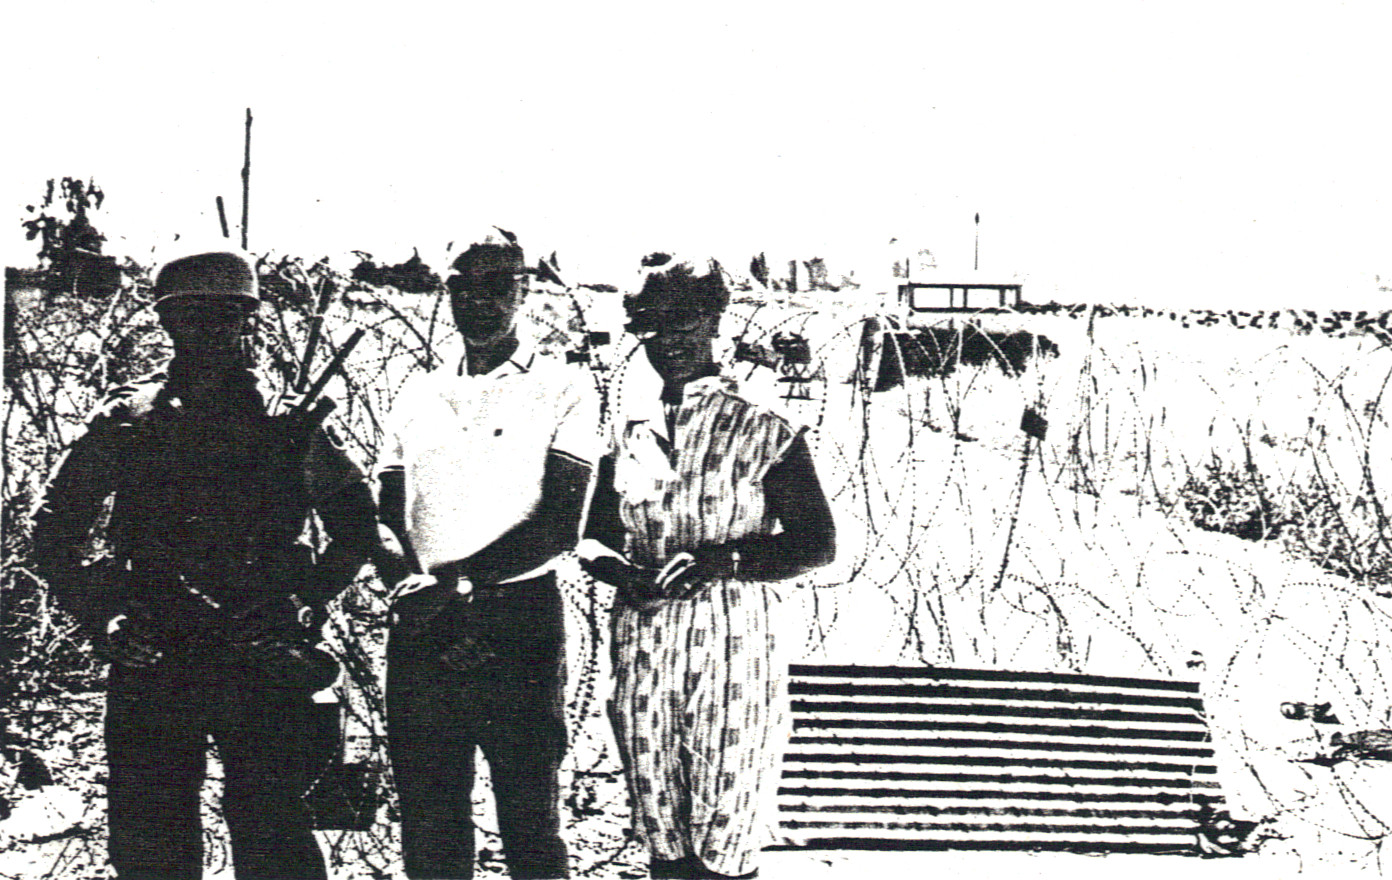
\includegraphics[width=0.9\textwidth]{photos/israel1}
  \caption{With Austrian guard at Israel-Syria border.}
  \label{israel1}
\end{figure}

All was very quiet and peaceful (apart from the strong wind which was
blowing that day) but this had been the scene of terrible battles
during the 6-day war when the Israelis were desperate to re-capture
the last area of the Golan Heights. Near here we saw the sad remains
of the Syrian Headquarters up whose steps the Israelis had driven
their huge tanks in a bid to storm and capture the Headquarters. They
succeeded.

From here there were extensive views all around but the air was quite
cold.

We proceeded to Masada, a rather different Masada from the place of
the same name on the Dead Sea and pronounced differently. This Masada
has the accent on the first ``A'' but the second ``A'' of the Masada
Fortress is accentuated.

We were to pass through lovely apple growing country and these apples
are among the nicest in the world. What a land of contrasts Israel is
-- from the point of view of cultivation alone. Obviously then, there
is a great variation of climate even in such a small country.

We came to the town of Majdal Shams which is in the centre of the
apple-growing industry and is really busy and thriving and occupied
largely, by the Druze people. The Druze are Arabs who have formed
their own sect. They are still Moslem but have differing beliefs --
for instance they believe that the next Messiah will be born of a man
and, with this in view, the men wear very baggy black trousers to make
room for the baby who might be born to the lucky one. When I said
something about the facts of life, Teddy turned the full impact of
these enormously blue eyes on me and asked if there was any more of a
``way out'' theory than the way in which our Messiah was
conceived. This was neither the time nor the place to enter into a
discussion of that nature but I could see his point of view.  Because
of the income derived from the apple industry the people here are very
rich and we saw lovely homes overlooking delightful scenery in this
high and healthy environment.  In the distance we could see Mount
Hermon (9200~ft high) whose snows help to swell the Jordan river.
This is the very high peak which is the cornerstone of Israel, Syria
and Lebanon.

We went on to Metulla and stood by the ``Good Fence'' the other side
of which is Lebanon. All was quiet and undisturbed. Teddy took a
photograph of us there (see Picture~\ref{israel2}).

\begin{figure}
  \centering
  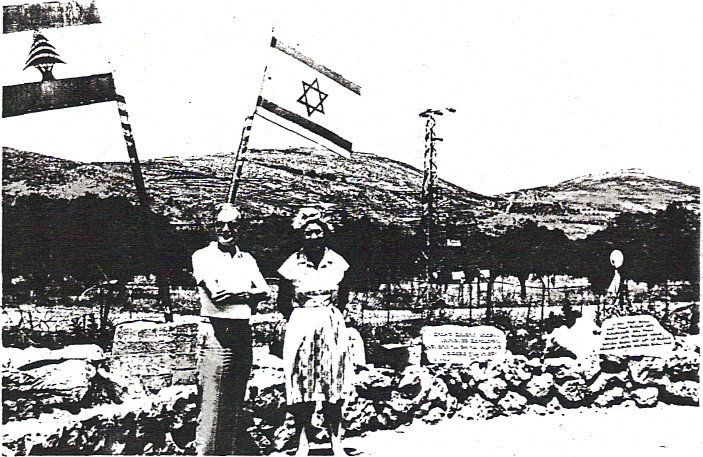
\includegraphics[width=0.9\textwidth]{photos/israel2}
  \caption{At the ``Good Fence'', bordering Lebanon.}
  \label{israel2}
\end{figure}

We were impressed by the leisurely atmosphere and old world charm of
Metullah but it must have been the centre of some very traumatic
incidents during recent wars.

On the way down from Metullah we passed Belinas, a Crusader Fort and
for quite a long time, we had lovely views of the Huleh Valley which
is extremely fertile and boasts many kibbuizim whose people look after
the crops.

We passed close by Kiryat Shmona named for the national hero, Joseph
Trumpeldor and his seven companions who, in 1920, died at the hands of
Arabs attacking the settlement of Tel Hai. The road passed very close
to the Lebanese border and we thought that Lebanon looked very
beautiful and certainly peaceful. We were now on the way to Rosh Pina
and from there to the Mount of the Beatitudes where Jesus preached the
sermon on the mount. As usual, on the site of a famous happening, a
church has been built and this again is a lovely one and in an
octagonal design; nearby is a rest house run by Franciscans. It was
amazing to hear Teddy talking to one of the Nuns in fluent Italian --
what a versatile man he is! Once more we saw beautiful and ancient
mosaics, this time mainly concentrated on the ceiling of the
church. Teddy persuaded one of the many tourists to take a photograph
of the three of us (see Picture~\ref{israel3}).

\begin{figure}
  \centering
  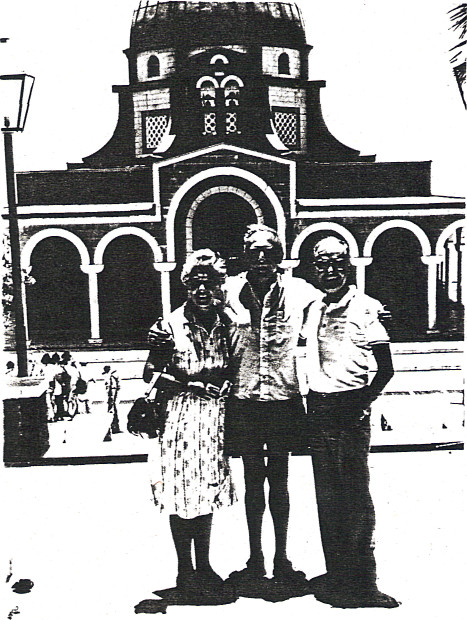
\includegraphics[width=0.9\textwidth]{photos/israel3}
  \caption{Madge, Teddy Vardi, and Tony at the church on the Mount of
    the Beatitudes.}
  \label{israel3}
\end{figure}

Soon we were on our way back to Tiberias - I think it was because we
had seen so much of interest that we seemed to have travelled further
than we did; in fact, we covered about 200~km that day and were to
travel approximately the same distance on the following day. We
stopped at a place called Banias which is one of the sources of the
River Jordan. Hillocks, rivulets and a lovely park create a beautiful
setting for the pagan temple of the God Pan whose image is carved in a
cave on the hill. We put our hands into the cool clear water.


\section{June 14th}

We got back to Tiberias tired but happy and on Thursday June 14th we
had to leave it -- Tiberias with its exquisite scenery, delicious
St. Peter's fish and unforgettable scenes of New Testament
reference. We promised to return some day!

We went on the road to Rosh Pina, the first of the Jewish settlements
in Galilee and, from there, to Safed. Teddy pronounced it Zfat and,
according to various signposts, it did seem to have several different
pronunciations to choose from.

Safed was entirely destroyed by an earthquake in 1836 but has been
charmingly rebuilt with colleges and art galleries etc.

The view from the car as we climbed up to Safed was breathtaking and
we felt the temperature falling which was welcome as the day was
already hot. The air was cool and invigorating and it is not
surprising that people visit this place to convalesce as there is a
Health giving spa as well as the superb climate. The wind sighing
through the pine trees was the sound of music.

Safed was once a fortress, not surprising in view of its high key
position, but now it is the home of students of the Cabbala a
mediaeval philosophy of direct communication between Man and God. We
visited two synagogues, one to the memory of Joseph Caro, a remowned
Rabbi and Scholar. Both the synagogues were small but quite exquisite.

Tony and I wandered through an Art Gallery but we were not inspired by
the Israeli style of Art either here or in any of the other galleries
we visited. Chagall is a different ``kettle of fish'' altogether.

It seemed a shame to have to leave the cool and invigorating
atmosphere of Safed and descend to the heat of the valley but we now
looked forward to our first visit to a Kibbutz -- Kibbutz Sasa --
which Teddy had helped to start and where he had lived for 8 years.

The kibbutz system is Communism with a small ``c'' and outside of
Israel, people seem to be very sceptical about it but it really does
seem to work with all the members, sometimes whole familes, of the
right mind to accept and contribute to the communal way of life. There
are strict rules of life and everything is well organised; if one
member shows any intellectual or any other kind of promise, funds are
used from the Kibbutz to further his education and some famous
Israelis started life in a kibbutz.

Teddy was thrilled to find that a new concert hall complete with
proper theatre type seats had been built since he was there. He was,
obviously, very proud of the place and it did look pretty and well
cared for. We got into chance conversation with a girl from Andover in
Hants -- once more a very small world!

Teddy promised to arrange for us to stay in a kibbutz next time; some
of them have well run guest houses which, of course, contribute to the
much needed income.

We proceeded on our way and saw signs to such places as Maalot, and
Nahariya but we were actually making for Acre which is Akko in the
Bible.

This interesting place attracted the first Canaanite settlers 4,000
years ago. It was fascinating to realise that there were several Acres
below the one upon which we walked and the history of it would take a
very long time to absorb -- it having passed through the rules of
Canaanites, Jews, Greeks, Romans, Crusaders, French, Turks etc., but
it would appear to the tourist that the Crusaders have left the
strongest mark although there is a very beautiful Turkish Mosque which
we did not have time to visit. It was with some awe that we were taken
to the subterranean Crypt of St. John and the Hospitaller, both of
which are absolutely huge and somehow, full of the atmosphere of
bygone days. We walked out on to the sea walk which of course provided
a grand view of the ancient Harbour (see Picture~\ref{israel4}).

\begin{figure}
  \centering
  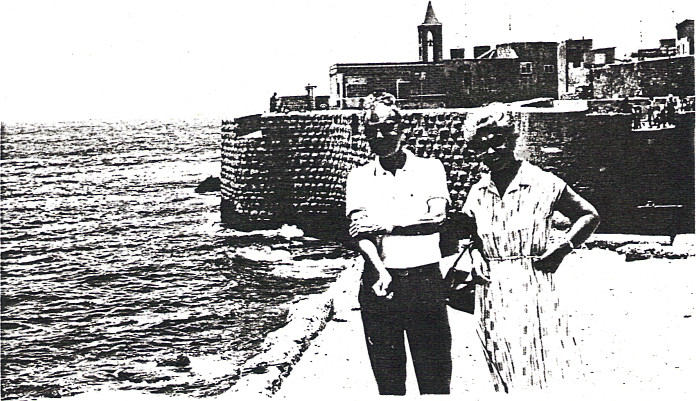
\includegraphics[width=0.9\textwidth]{photos/israel4}
  \caption{Tony and Madge beside the harbour at Acre.}
  \label{israel4}
\end{figure}

We would have enjoyed a much longer sojourn in Acre but time was
pressing. I felt that the volume of history was just crying out to be
absorbed but, unfortunately, we had to be on the move -- perhaps there
will be another occasion to visit Acre.

In the car again and on our way to Megiddo, we could see the Port of
Haifa on the opposite Point of the Bay as we passed below
Mt. Carmel. Megiddo is destined to be the site of the Final battle
between Good and Evil and Armageddon is the name given to this battle.

There has been expert and unbelievable excavation carried out by the
Oriental Institute of the University of Chicago and, at one place, it
is possible to look down a "Cut" and see 16 layers of civilization;
this was just too much to take in!

The energy and patience of archeologists are to be greatly admired and
it is not difficult to imagine the thrill and sense of achievement
asdf when some important discovery is made.

We found it paid dividends to examine the beautiful model of Megiddo,
ancient walled city of the 15th Century, BCE, before walking round the
site. This made the discovery of the partially restored walls, the
stepped water shaft leading to the water source, (unfortunately closed
on that day) the stables, palaces and storehouses much easier to
comprehend. It would have taken hours to explore the site for it is
huge. The heat was terrific in spite of the strong breeze. All around
us were extensive and lovely views and, Megiddo once having been a
hi11-Top Fortress, it was easy to see that it commanded a key position
and clear view of approaching enemies. On to Caesarea which boasts the
only Golf course in Israel! Caesarea was named for Augustus Caesar and
was under Roman rule for 600 years. From here St.~Paul set out for
some of his missions abroad. Once more, the Crusaders left a very
strong mark.

Teddy took us to a place where there are the remains of statues --
mostly headless and armless -- remains of the Roman era. They had been
beautifully carved, the folds of the garments looking very real. Teddy
took a photograph of us there and it is to be hoped that our friends
will be able to distinguish us from the statues (see
Picture~\ref{israel5})!

\begin{figure}
  \centering
  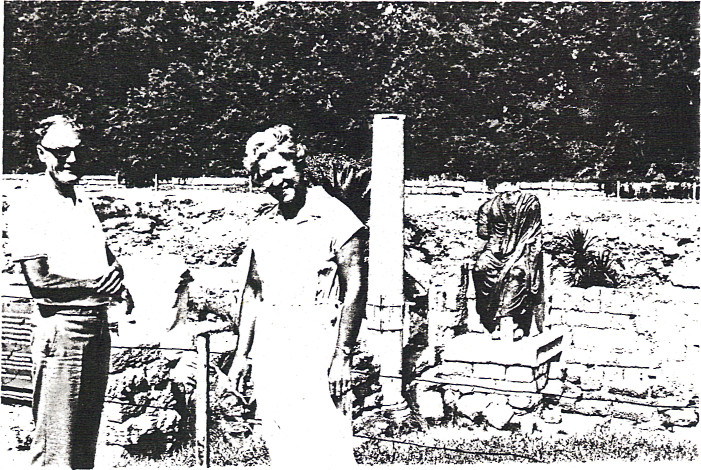
\includegraphics[width=0.9\textwidth]{photos/israel5}
  \caption{Tony and Madge beside statues at Caesarea.}
  \label{israel5}
\end{figure}

On to Natanya, the centre of Israel's diamond industry and the home of
the largest diamond exchange in the world. In this building we were
invited to watch a film about diamonds, which was very interesting,
and to observe some craftsmen filing those 58 facets on the precious
stones. Like a lot of very difficult crafts, it looked remarkably easy
and quick but it must take years of practice to develop such a skill.

It was interesting, and somewhat comforting -- to learn that it is
impossible for diamonds to lose their value; they can only appreciate
with time. We were taken to a lovely showroom where magnificent pieces
of finished jewellery were on display. One was now encouraged to buy
and some tourists were doing so but we were not certain of our dollars
even though we were coming to the end of our holiday. We had several
accounts still to settle and it would have been unwise to overspend at
this stage -- even so there were some ``mouth watering'' pieces to be
seen.

So firmly into the car and back ``home'' to Tel Aviv where we again
booked into the lovely ``Sheraton''. After some refreshments, we
regretfully had to say ``Goodbye'' to Teddy who had become a real
friend and companion during our travels together as well as being a
fantastic source of information. We felt sad at seeing him off but I
am sure this was not the end of our association. I do wonder what he
would think of what I have written...

I must admit to feeling a little lost back in Tel Aviv for we had
suddenly come to the end of culture and history and had absorbed a
surfeit of it but it was nice, after all, to look at the beautiful
Mediterranean from our balcony and to listen to the ever attractive
sounds of the sea. We had had a full day and had spent a lot of it in
the full blast of the sun which always induces tiredness, so after
baths and a customary stroll along the beach, we had a light supper
and went to bed quite early.


\section{June 15th}

Tony had business to do with the Telrad people on Friday morning, so I
used the time to catch up on my notes. I was going to wander to the
beach but it was suddenly lunchtime and Tony appeared to take me
downstairs to have something to eat.

We watched a video in the afternoon and then after the usual little
walk it was time to get ready for our Shabbat dinner invitation from
Gurion and Sara Meltzer.

As I have already written, this Friday night dinner is the highlight
of the week for Jewish families and it was therefore a great honour
for us, as Gentiles, to be invited.

Gurion and Sara are strict Orthodox Jews. Beno and Felya Ellman were
also invited and since they were coming to Johannesburg for a term of
duty shortly afterwards, it was pleasant to meet them beforehand, and
I suspect encouraging for them to know that there would be a least 2
familiar faces for them to see in an unfamiliar place. We liked them a
lot and, of course, Gurion and Sara are two of the most wonderful and
genuine people it is possible to meet.

We enjoyed Sara's delicious food and, throughout the meal, we were
fascinated by the rituals attached to it. Gurion explained each step
and ritual as we went along and the reasons why he blessed and
distributed the wine in a certain way and why a piece of bread was
cut for each member of the family whether they were present or
not. Prayers were said throughout the meal and with typical
thoughtfulness, Gurion provided us with prayer books in English so
that we would be able to follow the prayers which he was reciting oh!
so quickly.

This occasion was a memorable one for us; there was no restraint in
the conversation and the atmosphere was most friendly and
relaxed. Sara's mother, daughter and small grandson were present and
so it was a family occasion as well as being one to delight visitors.

The evening came to an end and we took our leave of them all with
thanks for allowing us to join them.


\section{June 16th}

Saturday was our last day in Israel and we had to decide what to do
with it but that did not take long. We would return to Jerusalem, a
distance of 50 km, and take a last fond look at the Old City. By this
time, it was evident that there would be dollars to spare for some
mementos of our visit so I decided that I would like to have the oil
lamp and filler I had seen in the Baidoun shop -- little did I know
that we would come away with a wine carafe as well.

The hotel doorman found us a very pleasant taxi driver who chatted to
us all the way to Jerusalem and promised to be waiting for us outside
the King David Hotel at a certain time -- and he was there on the dot.

Once more, Tony and I found great pleasure in walking though the Old
City, parts of which were by now, quite familiar to us. We found our
way to Mr Baidoun very easily and spent a pleasant hour chatting to
him and an American archeologist who assured us that anything we
bought in this shop was authentic -- indeed we were given certificates
of authenticity for our three purchases. How glad I am that we decided
to buy something worthwhile and valuable, there was so much ``junk''
there and I could not believe my eyes when I saw some Americans buying
``Crowns of Thorns''. Heaven knows how much they paid for them.

This had to be our final ``Farewell'' to the Old City and to
Jerusalem. I had so enjoyed my visits there and can still remember it
all vividly. Of the great number of impressions to be gained, I
believe that my chief one is amazement at the religious tolerance
which abounds. This, after all, is the home of the three great faiths,
all apparently living comfortably side by side... and Ireland cannot
cope with 2 offshoots of the same one!

The last evening in Tel Aviv was spent in the company of Gurion, Sara,
Ami and Osnat, for we had invited them to have dinner with us at our
hotel in the ``Twelve Tribes'' restaurant.

This was a lovely and enjoyable climax to our holiday and, of course,
they were all eager to learn of our impressions of their fabulous
country; naturally we were able to assure them that we were delighted
with everything we had seen and that we hoped, one. day, to return and
see those parts of Israel we had not had time to explore.

A lovely evening with good company, and good food in pleasant
surroundings is hard to beat.

Eventually we took our leave of them with promises to meet again
either in Israel or South Africa.

A lovely flight the next day by El Al to London and the start of
another glorious holiday but with so many memories of a happy time.

May we return one day.

\clearpage
\thispagestyle{empty}
